\section{Diagrama de Gantt}
Através das histórias de usuário geradas, foram extraídas atividades que compõem as funcionalidades desejadas. Com essas atividades, foi feito o diagrama de Gantt do projeto, onde as tarefas foram distribuídas de maneira visual entre as sprints do grupo, a fim de organizar o cronograma de desenvolvimento. 

\begin{figure}[H]
  \centering
  \caption{Diagrama de Gantt}
  \label{fig:cli-srv}
  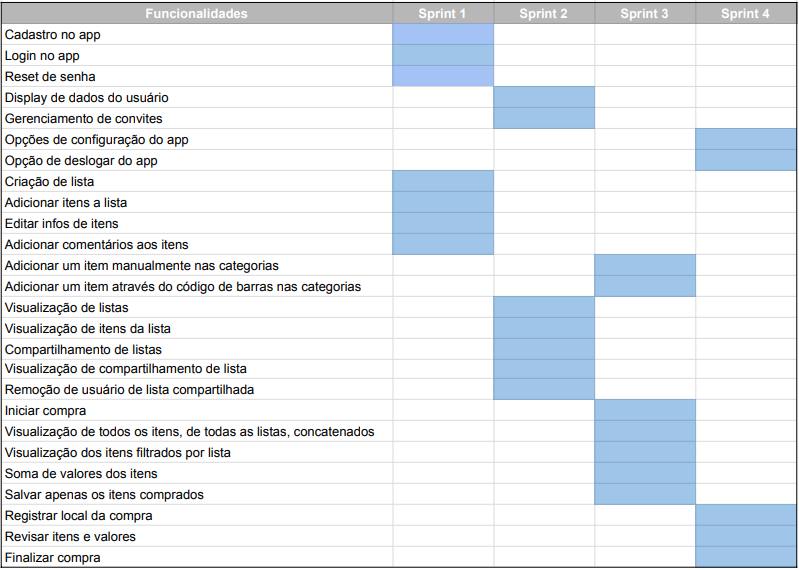
\includegraphics[scale=0.7]{Gantt}
	\fonte{Os Autores}
\end{figure}
